\documentclass[dvips,xcolor=pst]{beamer}
%\documentclass[dvips,handout,xcolor=pst]{beamer}
%\documentclass[letterpaper]{article}
%\usepackage{beamerarticle}
\newcommand{\newblock}{}
\usepackage{pstricks}
%\usepackage{hyperref}
%\usepackage[authoryear]{natbib}
\usepackage{graphicx}
\usepackage{multimedia}
\usepackage{pgfpages}
\usepackage{arydshln}
\usepackage{commath}
\usepackage{vector}
%\usepackage{cancel}
\usepackage{ulem}
\usepackage{listings}
%\usepackage{times}

\graphicspath{{pysci_eps/}}

\newcommand{\defeq}{\ensuremath{\buildrel {\text{def}}\over{=}}} 

%\usetheme{Berlin}
%\usetheme{Boadilla}
%\usetheme{Luebeck}
%\usetheme{Pittsburgh}
\usetheme{CambridgeUS}
%\usecolortheme{seagull}
%\setbeameroption{show notes}
%\setbeameroption{show only notes}
%\pgfpagesuselayout{2 on 1}[letterpaper,border shrink=0.2in]
%\usefonttheme[stillsansseriftext]{serif}
\usefonttheme[onlymath]{serif}

\title[Futuristic Computing with Python]{Futuristic Computing Platform for
Science and Engineering: Python + NumPy/SciPy/Matplotlib}
%
\author[\href{http://solvcon.net/yyc/}{Chen}]%
{\href{http://solvcon.net/yyc/}{Yung-Yu Chen} \\ {\scriptsize
\url{yyc@solvcon.net}}}
%
%\institute[\href{http://solvcon.net/}{SOLVCON}]%
%{\href{http://solvcon.net/}{SOLVCON Project}}
\institute[PyHUG]{Python Hsinchu User Group}
%
\date[2011/9/19]{September 19, 2011}

\begin{document}

\begin{frame}
\titlepage
\end{frame}

\section{
%%%
Futuristic Scientific Computing
%%%
}

\begin{frame}{
%
Python for Scientific and Engineering Computing
%
} \large
Python shows the traits of a futuristic computing platform for scientific and
engineering applications:
\begin{itemize} \large
  \item Productive.
  \begin{itemize} \large
    \item Concise syntax for rapid development.
    \item Versatile in built-in and 3rd-party libraries.
    \item Short time to delivery.
  \end{itemize}
  \item Robust and maintainable.
  \begin{itemize} \large
    \item Deliver correct and easy-to-be-maintained code.
  \end{itemize}
  \item Reasonably fast.
  \begin{itemize} \large
    \item Avoid performance penalties.
    \item I/O intensive: Pure Python is sufficient.
    \item Computational intensive: Easy to be optimized by using C or Fortran.
  \end{itemize}
\end{itemize}
\end{frame}

\begin{frame}{
%
Basic Python Scientific Tool Chain
%
}
\begin{itemize} \large
  \item NumPy: \url{http://numpy.scipy.org/}
  \begin{itemize} \large
    \item The core part is N-dimensional arrays, which are defined in
    \texttt{numpy.ndarray}.
    \item The N-dimensional arrays serve as the foundation for all
    scientific computing tasks in Python.
  \end{itemize}
  \item SciPy: \url{http://www.scipy.org/}
  \begin{itemize} \large
    \item Provide calculation functionalities for scientific computing tasks,
    including: Linear algebra, equation solving, ODE integration,
    interpolation, special functions, Fourier transform, signal processing,
    etc.
  \end{itemize}
  \item Matplotlib: \url{http://matplotlib.sourceforge.net/}
  \begin{itemize} \large
    \item Two-dimensional plotting: Line, polar, bar, X-Y, pie, etc.
  \end{itemize}
\end{itemize}
\end{frame}

\begin{frame}{
%
Python + NumPy + SciPy + MPL = Better MxxLAB
%
}
\begin{itemize} \large
  \item The basic layer: (i) Array operation (NumPy), (ii) calculation tools
  (SciPy), and (iii) visualization/presentation (Matplotlib).
  \item Advanced tools:
  \begin{itemize} \large
    \item Complementary functionalities to SciPy: SciKits
    (\url{http://scikits.appspot.com/}).
    \item Symbolic mathematics: SymPy (\url{http://sympy.org/}).
    \item Statistical computing: statlib
    (\url{http://code.google.com/p/python-statlib/}).
    \item General-purpose GPU computing:
    \href{http://mathema.tician.de/software/pycuda}{PyCUDA} and
    \href{http://mathema.tician.de/software/pyopencl}{PyOpenCL}.
  \end{itemize}
\end{itemize}
\end{frame}

\begin{frame}{
%
Python Facilitates Software Engineering
%
}
\begin{itemize} \large
  \item The language provides abundant armament for developing maintainable
  code.
  \begin{itemize} \large
    \item Multi-paradigm: object-oriented, procedural, and functional.
    \item Built-in containers: \texttt{dict}, \texttt{tuple}, \texttt{list}, 
    \texttt{set}, etc.
    \item Meta-classing.
  \end{itemize}
  \item Production tools:
  \begin{itemize} \large
    \item Documentation: docutils and sphinx.
    \item Unit tests: built-in framework and \texttt{nosetests}.
    \item Continuous integration: buildbot.
  \end{itemize}
\end{itemize}
\end{frame}

\begin{frame}{
%
Optimization by Using C
%
}
\begin{itemize} \large
  \item Use Python constructs.
  \begin{itemize} \large
    \item The operations of the built-in containers are implemented in C.
    \item \texttt{numpy.ndarray} supports many operations written in
    pre-compiled C code.
  \end{itemize}
  \item Write C code yourself.
  \begin{itemize} \large
    \item Develop a C extension.
    \item Use Cython.
    \item Write C and then load by using \texttt{ctypes}.
    \item Write C++ and then interface by using swig or boost.python.
  \end{itemize}
\end{itemize}
\end{frame}

\section{
%%%
Basic Layer
%%%
}

\subsection{
%%
NumPy
%%
}

\begin{frame}{
%
NumPy
%
}
\begin{itemize} \large
  \item Installation.
  \begin{itemize} \large
    \item Debian/Ubuntu: \texttt{apt-get install python-numpy}
    \item Windows: Enthought Python Distribution (EPD).
  \end{itemize}
  \item Every task starts with making a \texttt{ndarray} object.
  \begin{itemize} \large
    \item \texttt{import numpy as np}
    \item From existing data: \texttt{arr = np.array(list\_or\_tuple)}
    \item Create uniform data: \texttt{arr = np.zeros((dim1, dim2, dim3))}
    \item Allocate memory: \texttt{arr = np.empty((dim1, dim2), dtype='float64')}
  \end{itemize}
\end{itemize}
\end{frame}

\begin{frame}[fragile]{
%
Calculate Values of an Array
%
}
\begin{lstlisting}[language=Python]
>>> import numpy as np
>>> arr = np.array([1, 2, 3], dtype='float64')
>>> brr = np.array([4, 5, 6], dtype='float64')
>>> crr = arr + brr # create a new object.
>>> print crr
[ 5.  7.  9.]
>>> print id(arr), id(brr), id(crr)
44843680 44845952 44855776
>>> arr *= 2  # modify the current object.
>>> print arr
[ 2.  4.  6.]
>>> print id(arr)
44843680
\end{lstlisting}
\end{frame}

\begin{frame}[fragile]{
%
Array Manipulation
%
}
\small
\begin{lstlisting}[language=Python]
>>> mat = np.zeros((3,3), dtype='float64')
>>> mat[1,2] = 3
>>> print mat
[[ 0.  0.  0.]
 [ 0.  0.  3.]
 [ 0.  0.  0.]]
>>> mtt = mat.T # transpose.
>>> print mtt
[[ 0.  0.  0.]
 [ 0.  0.  0.]
 [ 0.  3.  0.]]
>>> mtt[0,1] = 5
>>> print mat
[[ 0.  0.  0.]
 [ 5.  0.  3.]
 [ 0.  0.  0.]]
\end{lstlisting}
\end{frame}

\subsection{
%%
SciPy
%%
}

\begin{frame}{
%
SciPy
%
}
\begin{itemize} \large
  \item Installation.
  \begin{itemize} \large
    \item Debian/Ubuntu: \texttt{apt-get install python-scipy}
    \item Windows: Enthought Python Distribution (EPD).
  \end{itemize}
  \item SciPy is a collection of tools.
  \item Each sub-package should be imported individually.
\end{itemize}
\end{frame}

\begin{frame}[fragile]{
%
Find Determinant
%
}
\begin{align*}
  A = \left(\begin{array}{ccc}
    1 & 1 & 4 \\ 1 & -1 & 3 \\ 2 & 0 & 1
  \end{array}\right) \quad \Rightarrow \quad
  \det(A) = 12
\end{align*}
\begin{lstlisting}[language=Python]
>>> import numpy as np
>>> from scipy import linalg
>>> A = np.array([[1, 1, 4], [1, -1, 3],
... [2, 0, 1]], dtype='float64')
>>> print linalg.det(A)
12.0
\end{lstlisting}
\end{frame}

\begin{frame}[fragile]{
%
Solve Eigen Problem
%
}
\begin{align*}
 &A = \left(\begin{array}{ccc}
    1 & 1 & 4 \\ 1 & -1 & 3 \\ 4 & 3 & 5
  \end{array}\right) \\
 &A\bvec{v} = \lambda\bvec{v} \Rightarrow A - \lambda I = 0
\end{align*}
where $\lambda$ is the eigenvalue and $\bvec{v}$ is the eigenvector of the
square matrix $A$.
\begin{lstlisting}[language=Python]
>>> import numpy as np
>>> from scipy import linalg
>>> A = np.array([[1, 1, 4], [1, -1, 3],
... [4, 3, 5]], dtype='float64')
>>> eval, evec = linalg.eig(A)
>>> print eval
[ 8.47722558+0.j -1.00000000+0.j -2.47722558+0.j]
\end{lstlisting}
\end{frame}

\subsection{
%%
Matplotlib
%%
}

\begin{frame}{
%
Matplotlib
%
}
\begin{itemize} \large
  \item Installation.
  \begin{itemize} \large
    \item Debian/Ubuntu: \texttt{apt-get install python-scipy}
    \item Windows: Enthought Python Distribution (EPD).
  \end{itemize}
  \item SciPy is a collection of tools.
  \item Each sub-package should be imported individually.
\end{itemize}
\end{frame}

\begin{frame}[fragile]{
%
Line Plot
%
}
\begin{columns}
\begin{column}{0.5\textwidth}
\lstinputlisting[language=Python]{plt1.py}
\end{column}
\begin{column}{0.5\textwidth}
  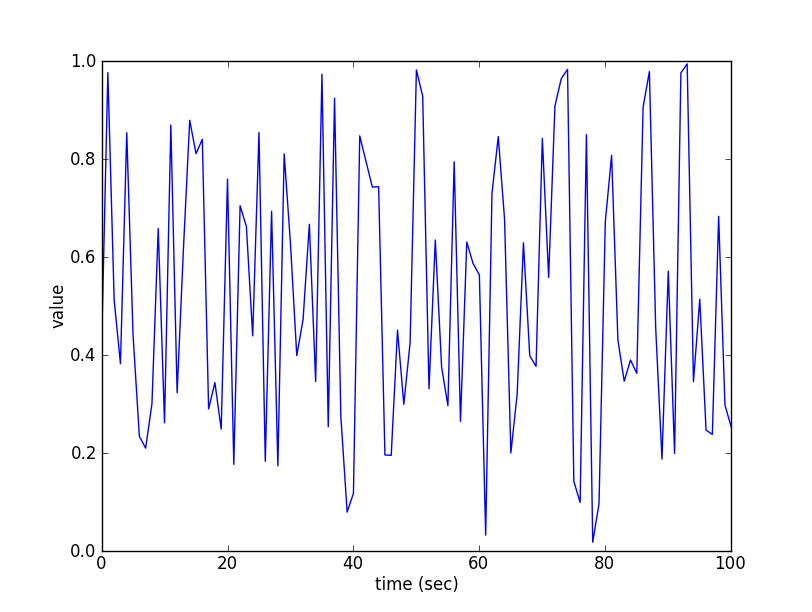
\includegraphics[width=\textwidth]{plt1.eps}
\end{column}
\end{columns}
\end{frame}

\begin{frame}[fragile]{
%
Sub-Plot
%
}
\begin{columns}
\begin{column}{0.5\textwidth}
\lstinputlisting[language=Python]{plt2.py}
\end{column}
\begin{column}{0.5\textwidth}
  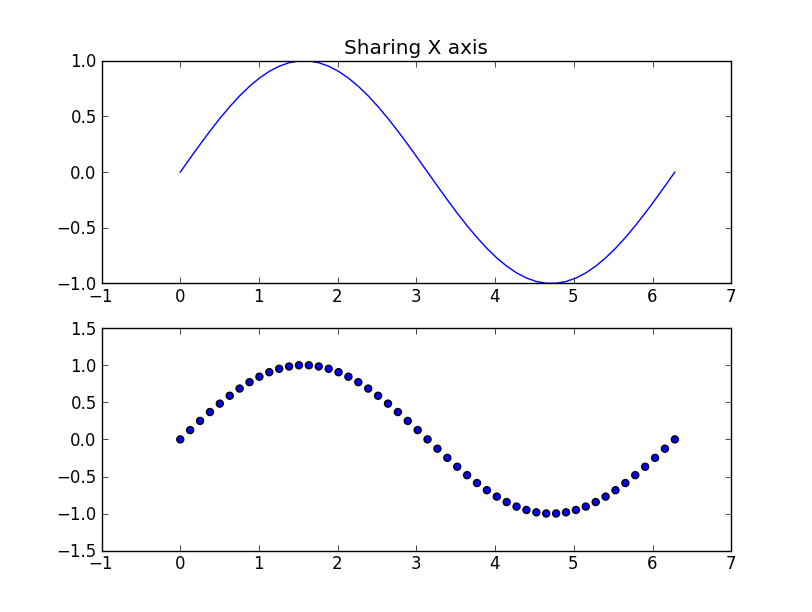
\includegraphics[width=\textwidth]{plt2.eps}
\end{column}
\end{columns}
\end{frame}

\subsection{
%%
Documentation
%%
}

\begin{frame}{
%
Documentation
%
}
\begin{itemize} \large
  \item NumPy and SciPy: \url{http://docs.scipy.org/doc/}
  \begin{itemize} \large
    \item NumPy book: \url{http://docs.scipy.org/doc/numpy/user/}
    \item NumPy reference: \url{http://docs.scipy.org/doc/numpy/reference/}
    \item SciPy reference: \url{http://docs.scipy.org/doc/scipy/reference/}
    \item Cookbook: \url{http://www.scipy.org/Cookbook}
  \end{itemize}
  \item Matplotlib: \url{http://matplotlib.sf.net/}
  \begin{itemize} \large
    \item Examples: \url{http://matplotlib.sf.net/examples/index.html}
  \end{itemize}
\end{itemize}
\end{frame}

\section{
%%%
High-Performance Computing
%%%
}

\begin{frame}{
%
Python for High-Performance Computing
%
}
\begin{center}
  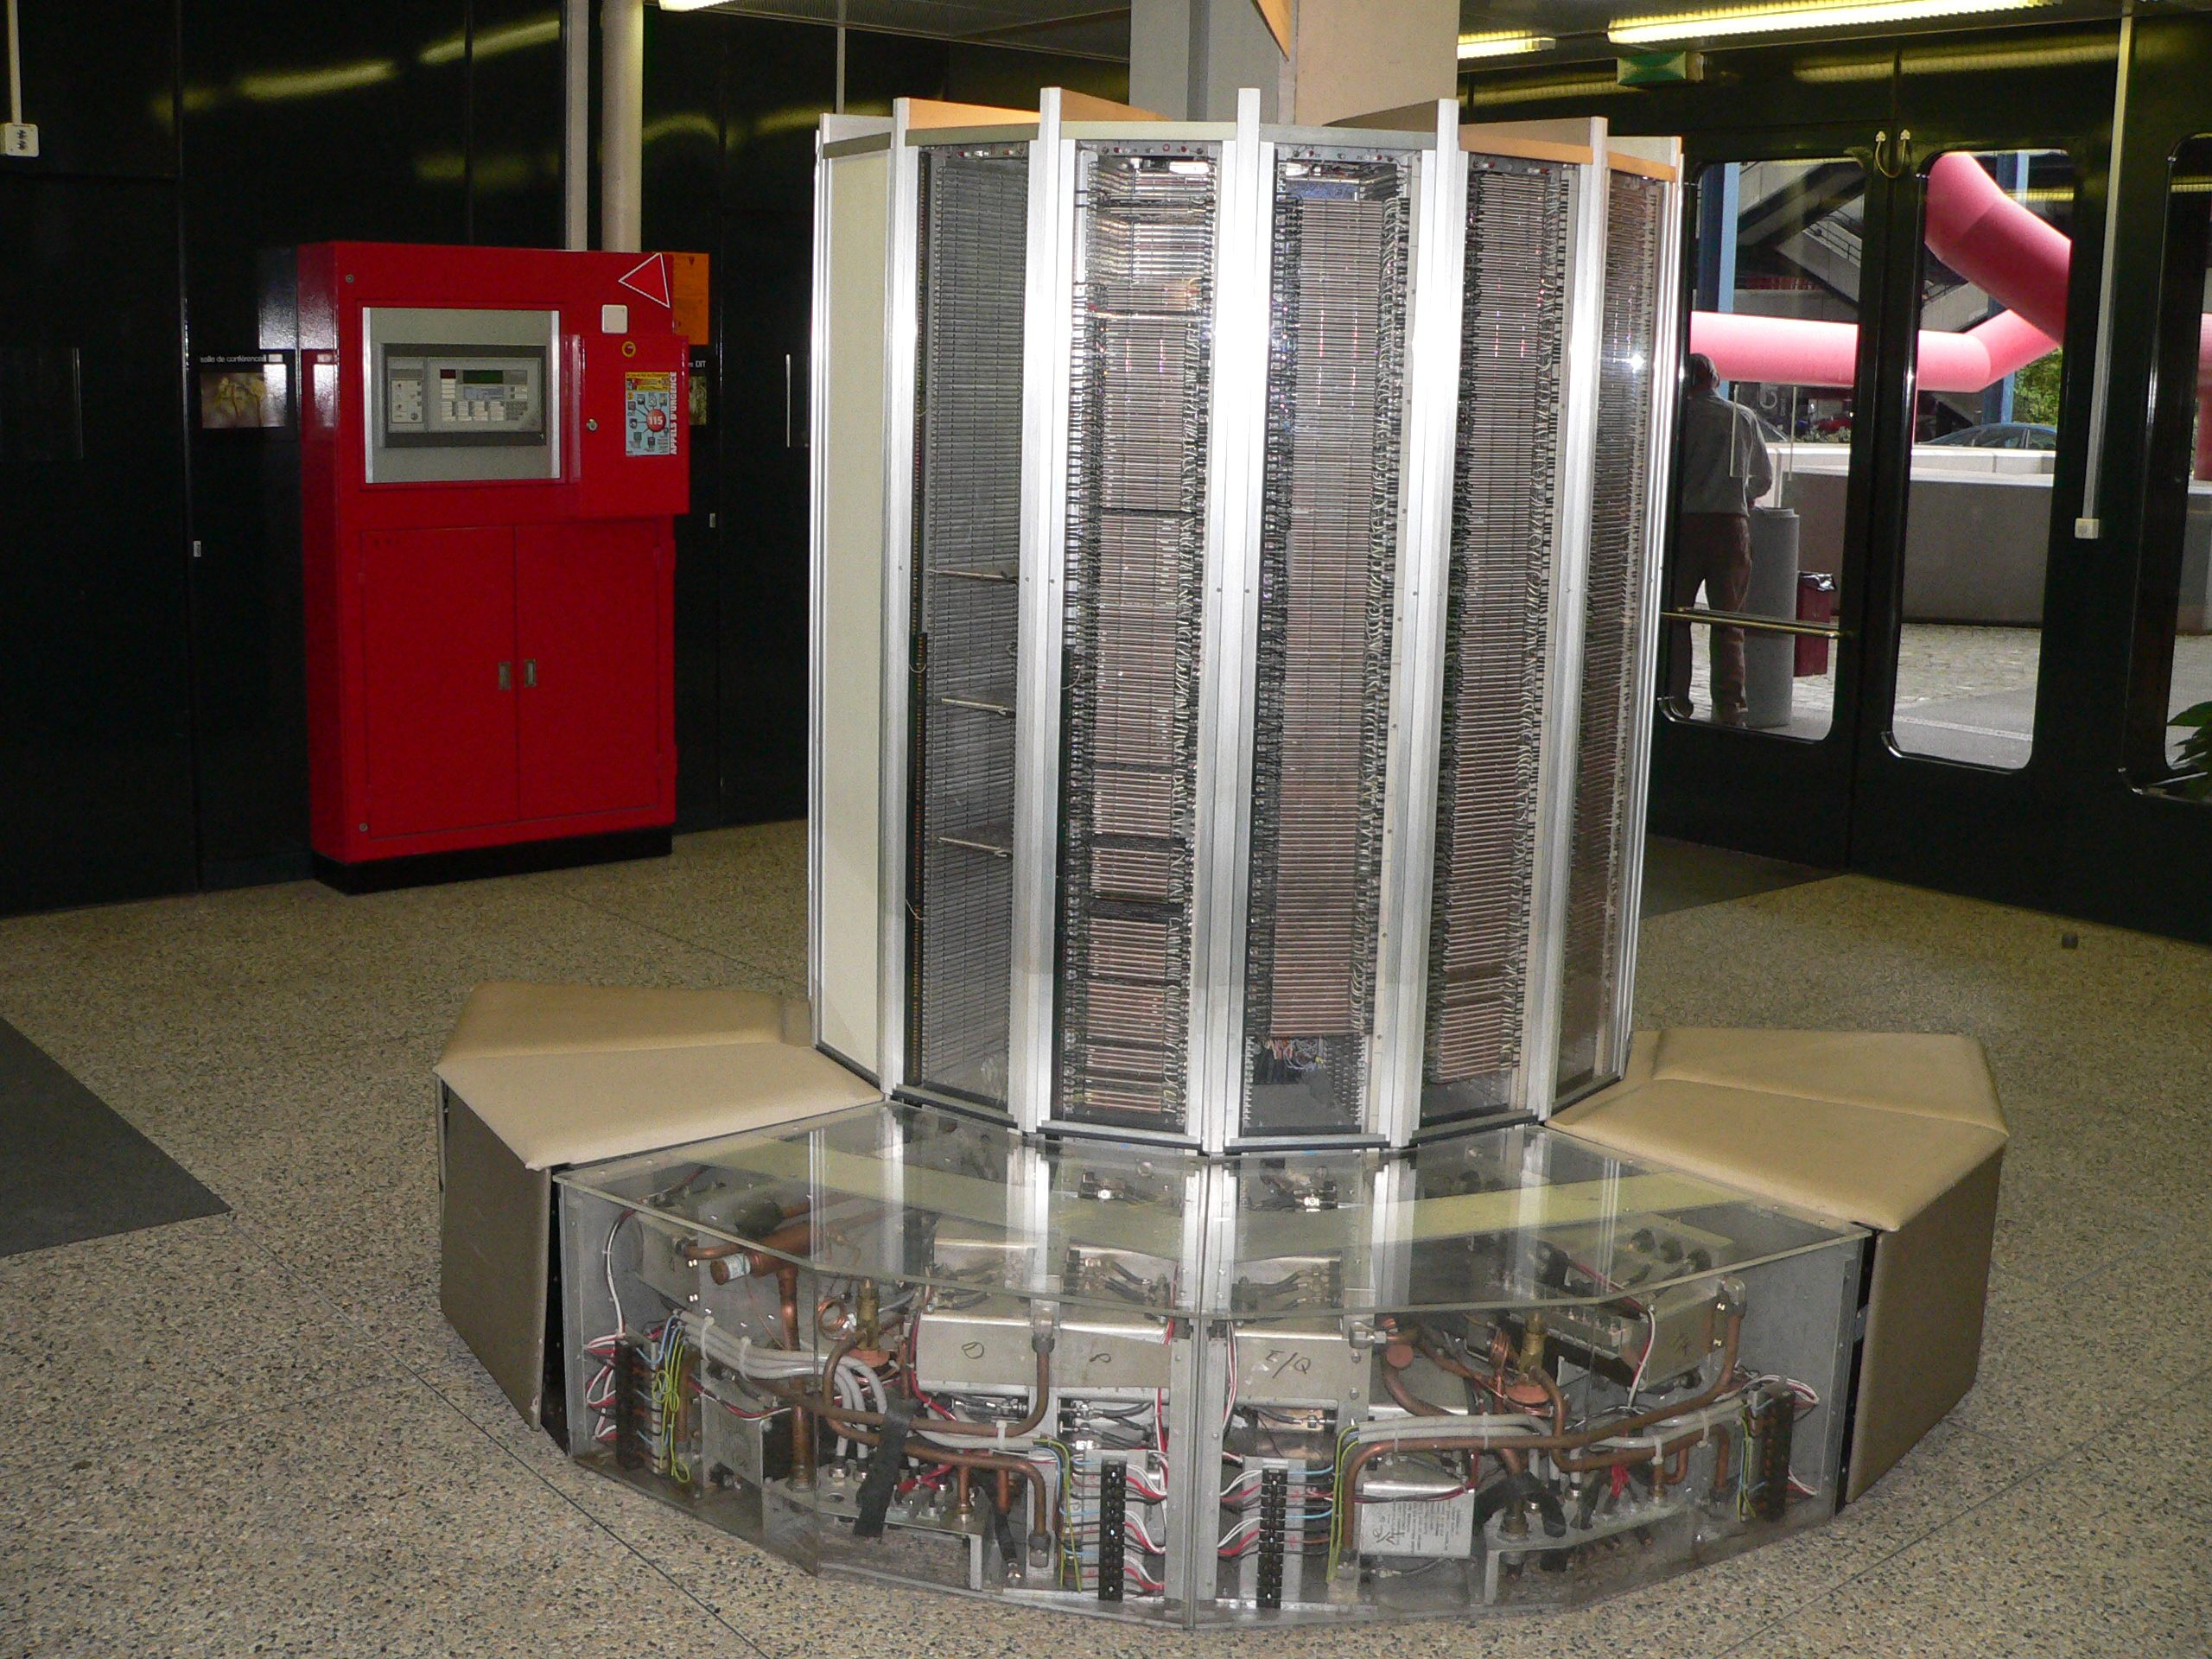
\includegraphics[height=0.3\textheight]{cray.eps}
  \hspace{0.01\textwidth}
  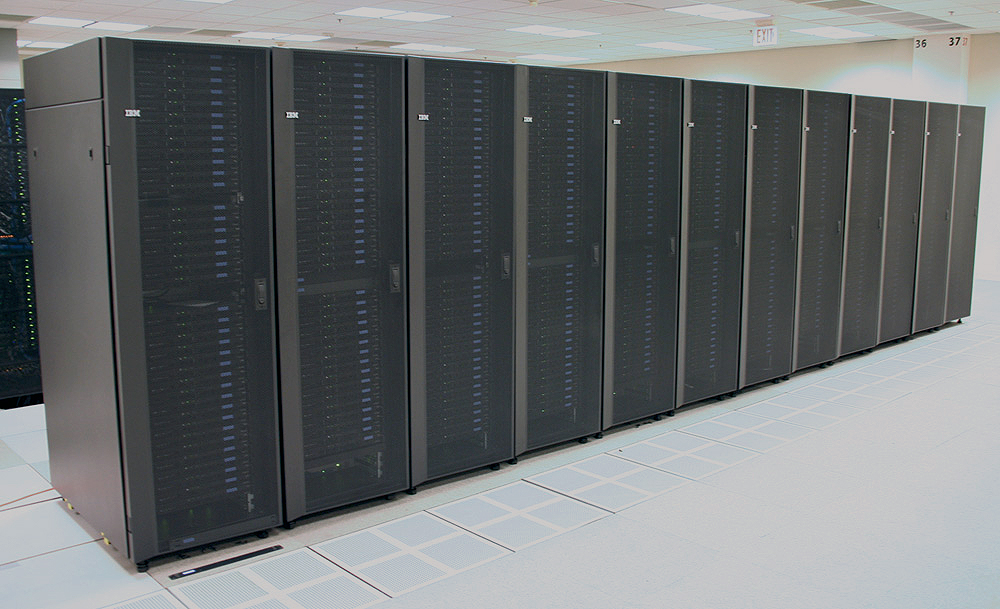
\includegraphics[height=0.3\textheight]{oscglenn.eps}
  \hspace{0.01\textwidth}
  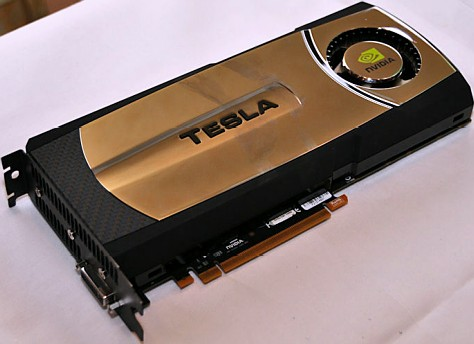
\includegraphics[height=0.3\textheight]{tesla_g300.eps}
\end{center}
\begin{itemize} \large
  \item New hardware boosts computing power.
  \begin{itemize} \large
    \item 1970-1990: Vector machines (Cray computers).
    \item 1990-200x: Clusters with MPI (10,000+ cores).
    \item Now: Many-core technology, e.g., general-purpose GPU clusters.
  \end{itemize}
  \item Quickly-evolving computer systems need agile programming for HPC
  software.
\end{itemize}
\end{frame}

\begin{frame}{
%
Hybrid Parallel Computing
%
}
\begin{minipage}[c]{\textwidth}\centering
\parbox{0.3\textwidth}{\centering
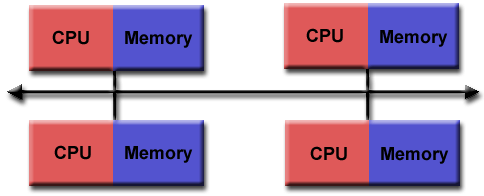
\includegraphics[width=0.3\textwidth]{mem_distributed.eps} \\ distributed
(cluster)}
+ 
\parbox{0.3\textwidth}{\centering 
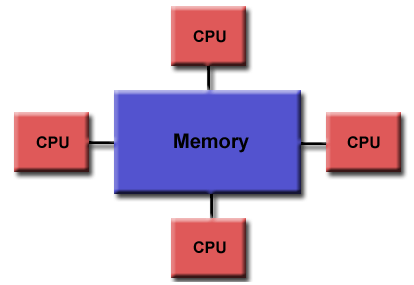
\includegraphics[width=0.3\textwidth]{mem_shared.eps} \\ shared (vector/GPU)}
= 
\parbox{0.3\textwidth}{\centering
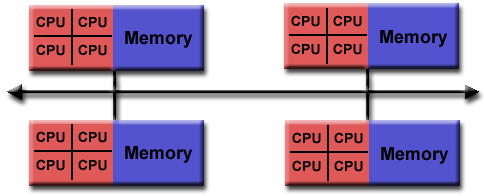
\includegraphics[width=0.3\textwidth]{mem_hybrid.eps} \\ hybrid (GPU cluster)}
\end{minipage}
\begin{itemize}
  \item Definition: Simultaneously use distributed-memory (e.g., MPI) and
  shared-memory (e.g., CUDA/OpenCL) parallel computing.
  \begin{itemize}
    \item The difference in parallel computing models requires using disparate
    programming tools.
  \end{itemize}
  \item A single language is not sufficient to model the hybrid system.
  \begin{itemize}
    \item None of C, C++, and Fortran alone can be productive.
    \item Software structure needs to be organized to accommodate the computing
    models.
  \end{itemize}
\end{itemize}
\end{frame}

\begin{frame}{
%
Example: Solving Conservation Laws
%
} \large
\begin{itemize}
  \item Three challenges for the next-generation solvers of conservation laws.
  \begin{itemize} \large
    \item Challenge 1: HPC by routinely using 1,000+ cores and GPGPU computing.
    \item Challenge 2: I/O and post-processing large data; the bottleneck is
    the laborious work flow for post-processing the results.
    \item Challenge 3: Code reuse for long life cycle.
  \end{itemize}
  \item Python can address the challenges.
  \begin{itemize} \large
    \item NumPy is the foundation.
    \item Replace the hotspots with C or CUDA code.
  \end{itemize}
\end{itemize}
\end{frame}

\section{Conclusions}

\begin{frame}{
%
Conclusions
%
}
\begin{itemize} \large
  \item De facto Python tool chain for scientific and engineering computing:
  NumPy + SciPy + Matplotlib.
  \begin{itemize} \large
    \item NumPy: The core of array operations.
    \item SciPy: Scientific calculations.
    \item Matplotlib: Two-dimensional plotting.
  \end{itemize}
  \item Python extends conventional scientific programming to use modern
  software-engineering practices.
  \item Python combined with C or CUDA: A productive approach to the best
  practice of HPC.
  \item Download the source files of the slides:
  {\small\url{https://bitbucket.org/yungyuc/talk/src/tip/20110919_pysci/}}
\end{itemize}
\end{frame}

\end{document}

% vim: set spell:
